\section{Die Funktionen}\label{sec:Die Funktion}
Eine Funktion ist eine Zuordnung aus zwei Zahlenmengen. Hierbei wird unterschieden zwischen Definitionsmenge und Wertemenge. Sei $a\in X$ und $b\in Y$, so bildet $a\rightarrow b$ ab, und stellt somit ein Zuordnung zweier Mengen dar. Hierbei wird jedem $x$ ein $y$ zu. 
%ToDo Die Definition sollte hier nochmals überarbeitet werden

\begin{beispiel} Fährt man mit einem Auto konstant 100km/h, so kann man dies auch in einer Wertetabelle darstellen. Hierbei ist zu beachten, dass die Funktion Kilometer in Zeit darstellt.
\begin{align*}
	1 \text{ Stunde}&\rightarrow100 \text{ Kilometer}\\
	2 \text{ Stunde}&\rightarrow200 \text{ Kilometer}\\
	3 \text{ Stunde}&\rightarrow300 \text{ Kilometer}\\
	4 \text{ Stunde}&\rightarrow400 \text{ Kilometer}
\end{align*}
\end{beispiel}
\subsection{Darstellung von Funktionen}\label{sec:Die Funktion/Darstellen von Funktionen}
Setzt man in eine Funktion für das $x$ einen Wert, so erhält man den zugehörigen $y$-Wert. Dieses Wertepaar lässt sich in ein Koordinatensystem eintragen(\ref{sec:Wertetabelle_einer_Funktion_visualisiert}). Verbindet man nun die Punkte miteinander, so entsteht der sogenannte Funktionsgraph. Auch lässt sich hierbei leicht erkennen, ob es sich überhaupt um eine Funktion, die eingetragen wurde, handelt. Betrachtet man die $Y$-Achse, als den obig erwähnten Wert und die $X$-Achse als Ausgangsmenge, so lässt sich feststellen, warum eine Funktion keine Zuweisung von zwei $X$-Werten haben kann.
\begin{figure}[h!]
\centering
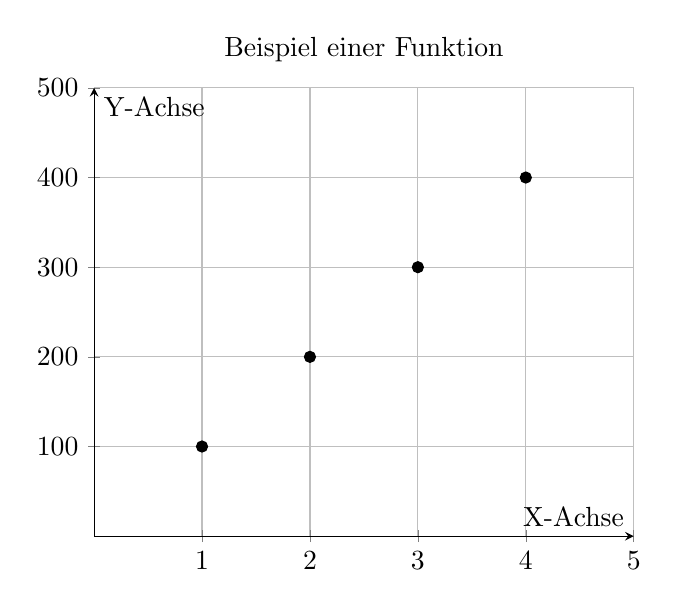
\begin{tikzpicture}
\begin{axis}[
    title={Beispiel einer Funktion},
    xlabel={X-Achse},
    ylabel={Y-Achse},
    axis lines=middle, % Zentriert die Achsen
    xmin=0, xmax=5, % Setzt die Grenzen für die X-Achse
    ymin=0, ymax=500, % Setzt die Grenzen für die Y-Achse
    grid=major, % Fügt ein Hauptgitter hinzu
]
\addplot[mark=*] coordinates {(1,100)};
\addplot[mark=*] coordinates {(2,200)};
\addplot[mark=*] coordinates {(3,300)};
\addplot[mark=*] coordinates {(4,400)};
\end{axis}
\end{tikzpicture}
\caption{Wertetabelle einer Funktion visualisiert}
\label{sec:Wertetabelle_einer_Funktion_visualisiert}
\end{figure}

 
